%
\clearpage
%
\section{Appendix}\label{sec:appendix}
%
\vspace{-20pt}
\begin{figure}[h!]
\begin{center}
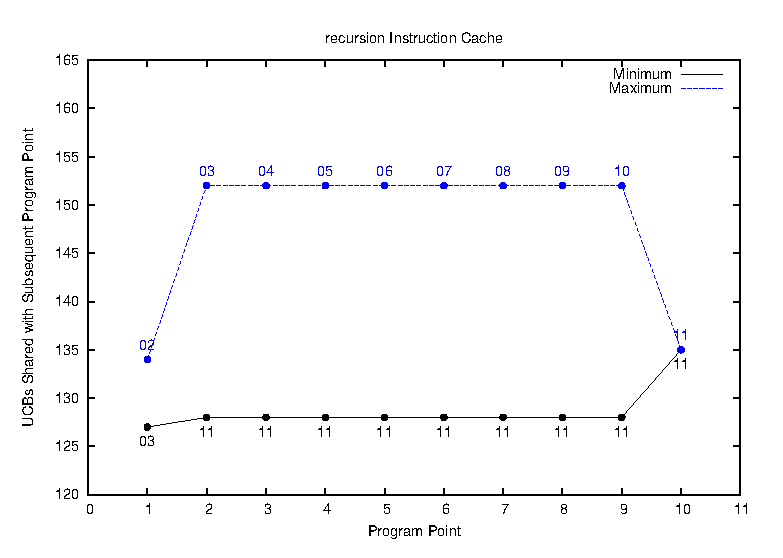
\includegraphics[width=\linewidth]{eps/recursion-icache.eps}
\caption{Recursion Instruction Cache.}
\label{fig:recursion_instruction_cache}
\end{center}
\end{figure}
%
\vspace{-20pt}
\begin{figure}[h!]
\begin{center}
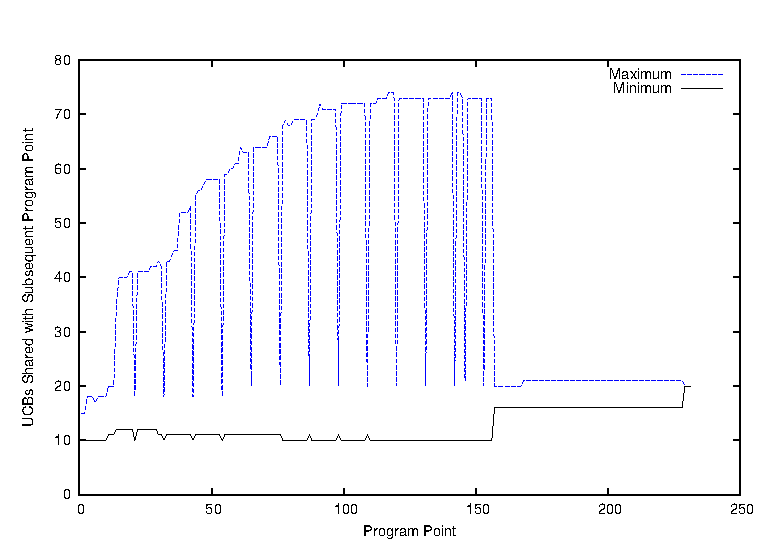
\includegraphics[width=\linewidth]{eps/adpcm-dcache.eps}
\caption{ADPCM Data Cache.}
\label{fig:adpcm_data_cache}
\end{center}
\end{figure}
%
\vspace{-20pt}
\begin{figure}[h!]
\begin{center}
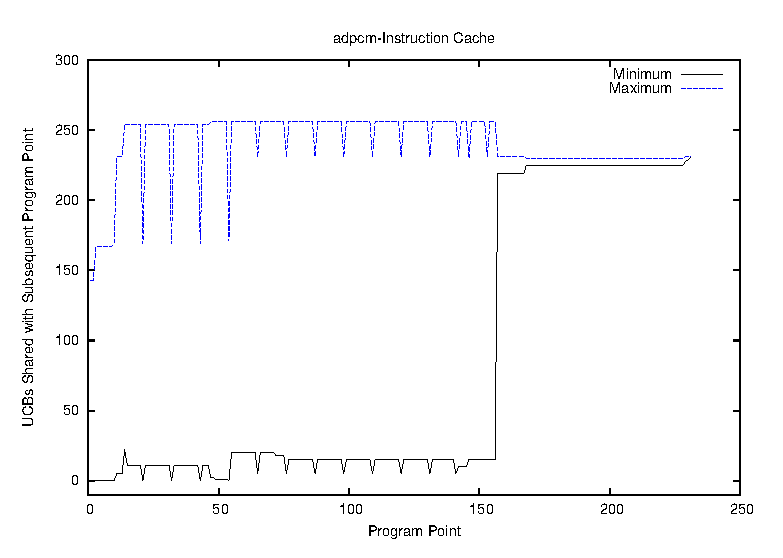
\includegraphics[width=\linewidth]{eps/adpcm-icache.eps}
\caption{ADPCM Instruction Cache.}
\label{fig:adpcm_instruction_cache}
\end{center}
\end{figure}
%
\vspace{-20pt}
\begin{figure}[h!]
\begin{center}
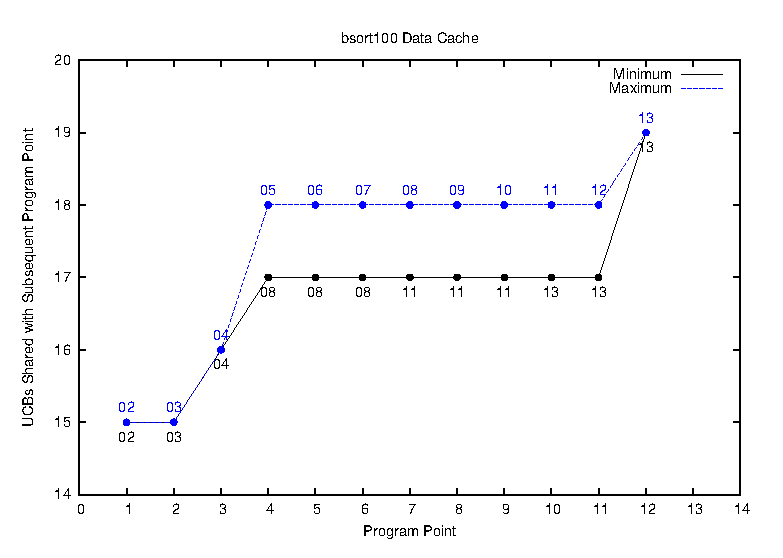
\includegraphics[width=\linewidth]{eps/bsort100-dcache.eps}
\caption{BSORT100 Data Cache.}
\label{fig:bsort100_data_cache}
\end{center}
\end{figure}
%
\vspace{-20pt}
\begin{figure}[h!]
\begin{center}
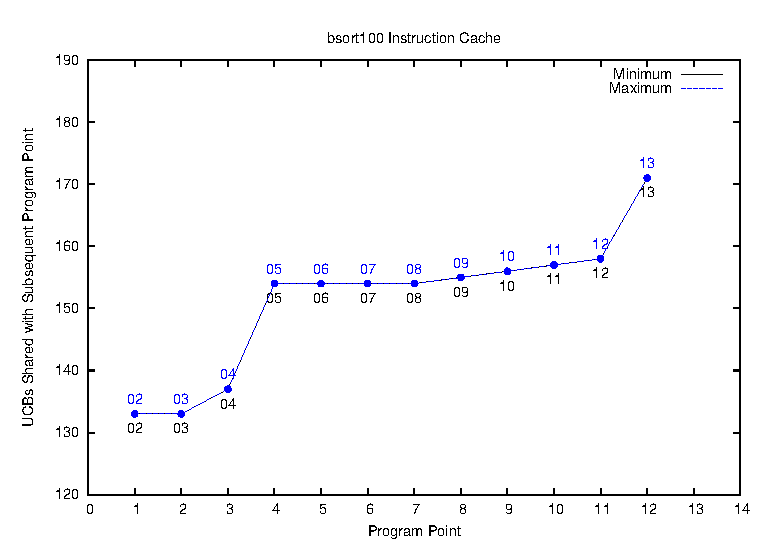
\includegraphics[width=\linewidth]{eps/bsort100-icache.eps}
\caption{BSORT100 Instruction Cache.}
\label{fig:bsort100_instruction_cache}
\end{center}
\end{figure}
%
\vspace{-20pt}
\begin{figure}[h!]
\begin{center}
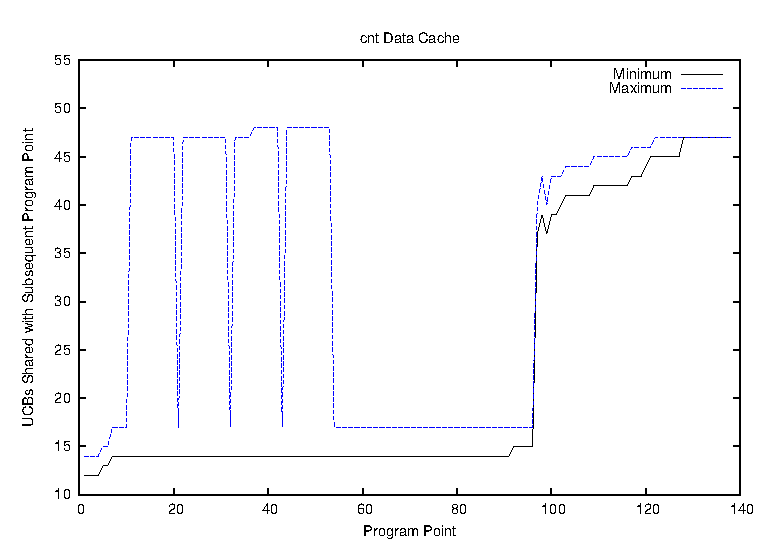
\includegraphics[width=\linewidth]{eps/cnt-dcache.eps}
\caption{CNT Data Cache.}
\label{fig:cnt_data_cache}
\end{center}
\end{figure}
%
\vspace{-20pt}
\begin{figure}[h!]
\begin{center}
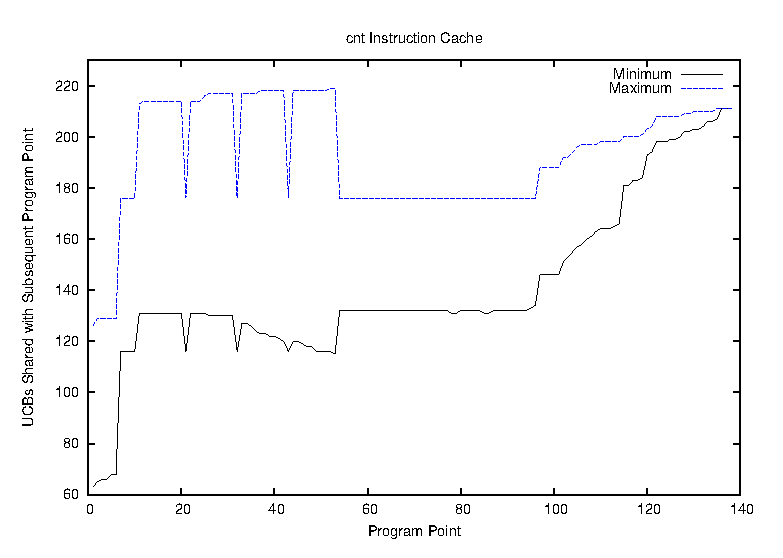
\includegraphics[width=\linewidth]{eps/cnt-icache.eps}
\caption{CNT Instruction Cache.}
\label{fig:cnt_instruction_cache}
\end{center}
\end{figure}
%
\vspace{-20pt}
\begin{figure}[h!]
\begin{center}
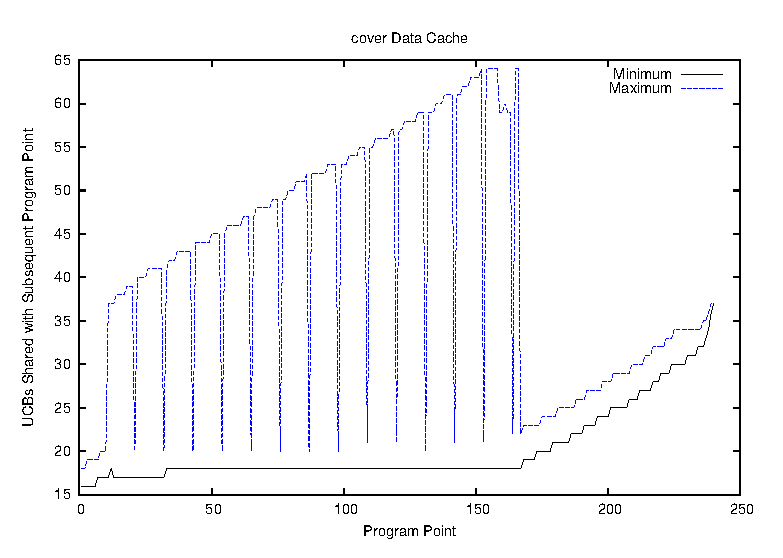
\includegraphics[width=\linewidth]{eps/cover-dcache.eps}
\caption{Cover Data Cache.}
\label{fig:cover_data_cache}
\end{center}
\end{figure}
%
\vspace{-20pt}
\begin{figure}[h!]
\begin{center}
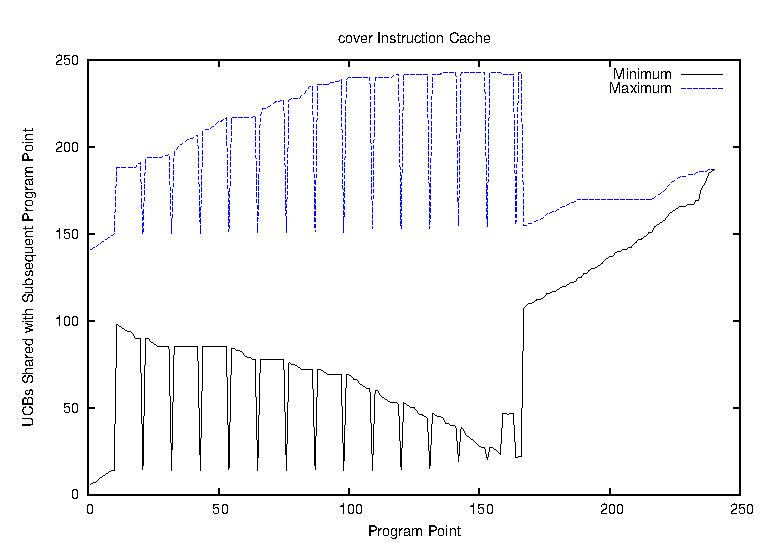
\includegraphics[width=\linewidth]{eps/cover-icache.eps}
\caption{Cover Instruction Cache.}
\label{fig:cover_instruction_cache}
\end{center}
\end{figure}
%
\vspace{-20pt}
\begin{figure}[h!]
\begin{center}
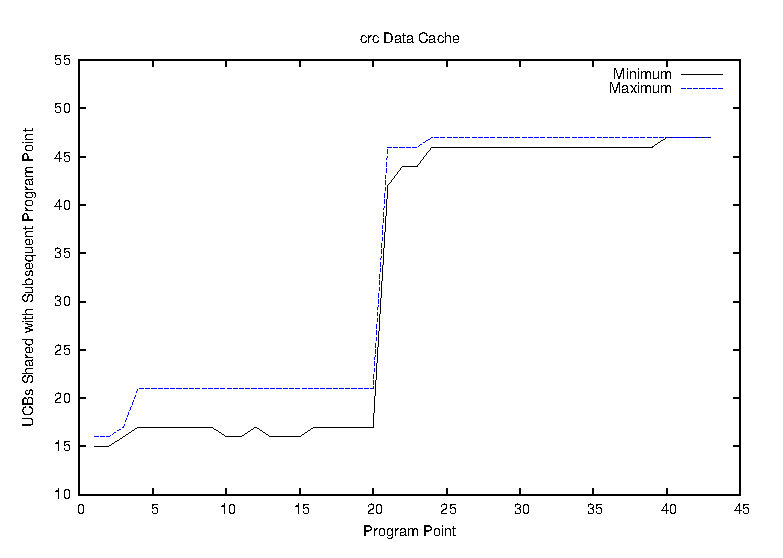
\includegraphics[width=\linewidth]{eps/crc-dcache.eps}
\caption{CRC Data Cache.}
\label{fig:crc_data_cache}
\end{center}
\end{figure}
%
\vspace{-20pt}
\begin{figure}[h!]
\begin{center}
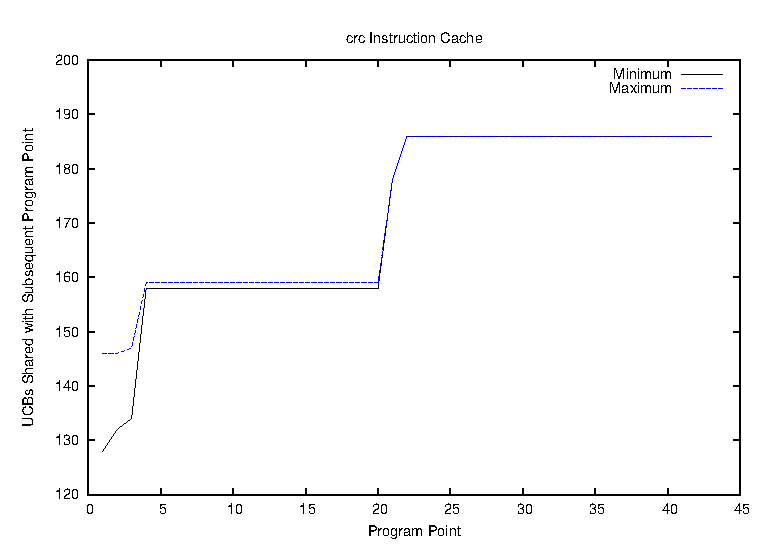
\includegraphics[width=\linewidth]{eps/crc-icache.eps}
\caption{CRC Instruction Cache.}
\label{fig:crc_instruction_cache}
\end{center}
\end{figure}
%
\vspace{-20pt}
\begin{figure}[h!]
\begin{center}
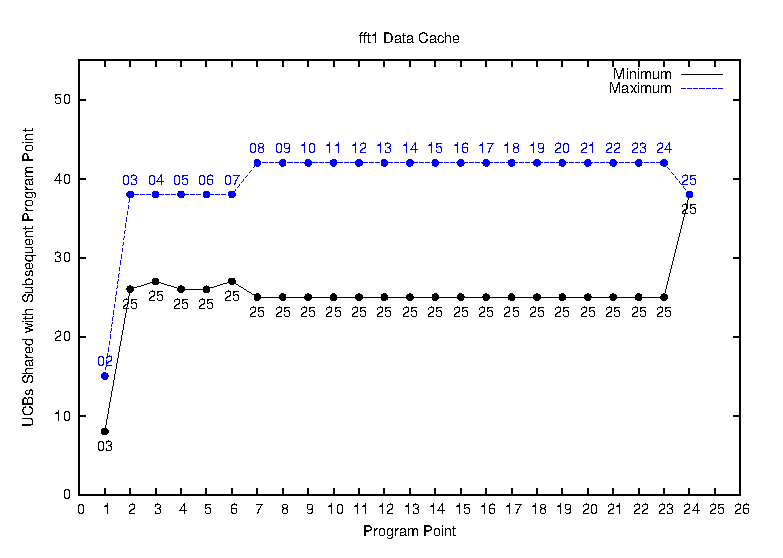
\includegraphics[width=\linewidth]{eps/fft1-dcache.eps}
\caption{FFT1 Data Cache.}
\label{fig:fft1_data_cache}
\end{center}
\end{figure}
%
\vspace{-20pt}
\begin{figure}[h!]
\begin{center}
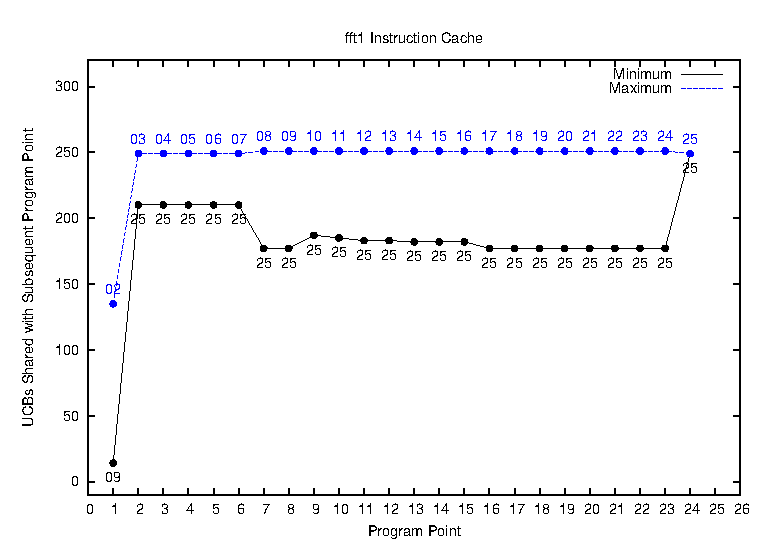
\includegraphics[width=\linewidth]{eps/fft1-icache.eps}
\caption{FFT1 Instruction Cache.}
\label{fig:fft1_instruction_cache}
\end{center}
\end{figure}
%
\vspace{-20pt}
\begin{figure}[h!]
\begin{center}
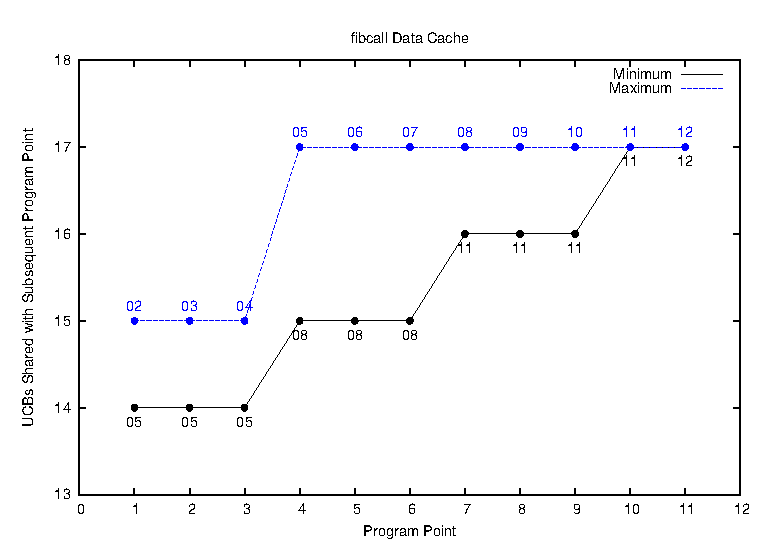
\includegraphics[width=\linewidth]{eps/fibcall-dcache.eps}
\caption{Fibcall Data Cache.}
\label{fig:fibcall_data_cache}
\end{center}
\end{figure}
%
\vspace{-20pt}
\begin{figure}[h!]
\begin{center}
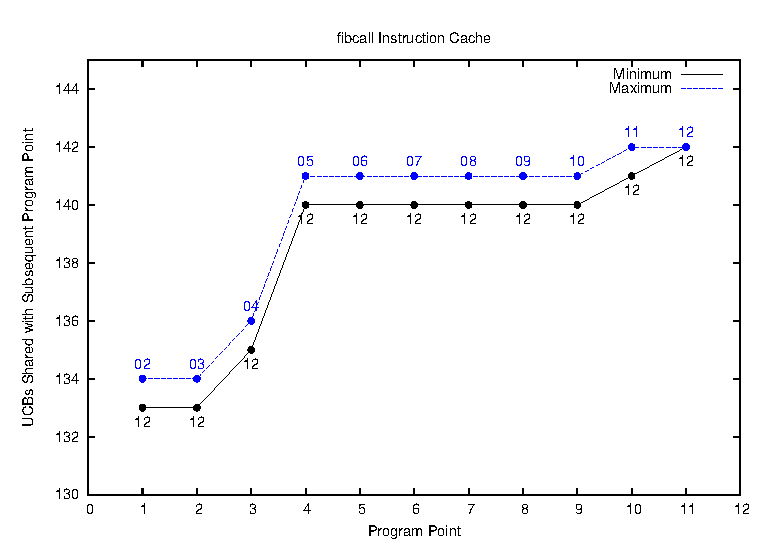
\includegraphics[width=\linewidth]{eps/fibcall-icache.eps}
\caption{Fibcall Instruction Cache.}
\label{fig:fibcall_instruction_cache}
\end{center}
\end{figure}
%
\begin{figure}[h!]
\vspace{-20pt}
\begin{center}
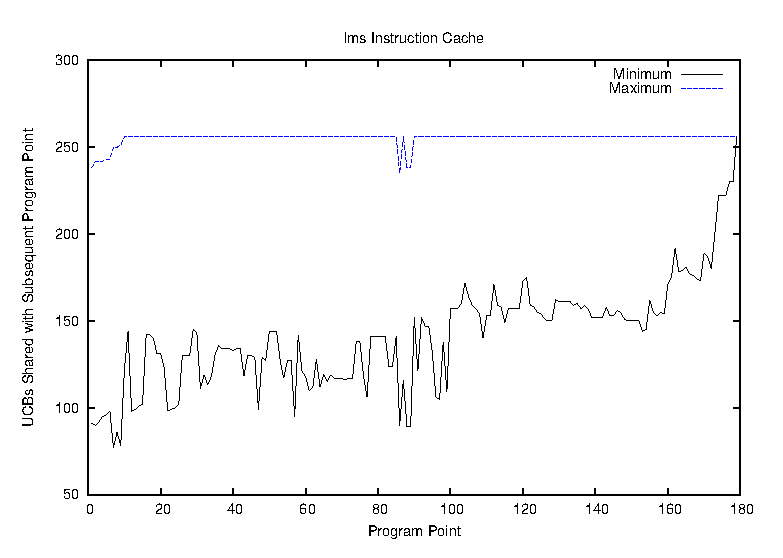
\includegraphics[width=\linewidth]{eps/lms-icache.eps}
\caption{LMS Instruction Cache.}
\label{fig:lms_instruction_cache}
\end{center}
\vspace{-10pt}
\end{figure}
%
\vspace{-20pt}
\begin{figure}[h!]
\begin{center}
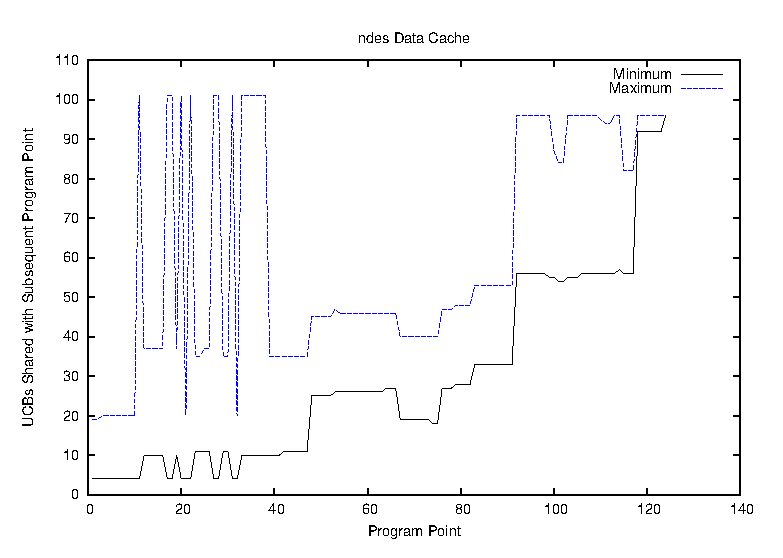
\includegraphics[width=\linewidth]{eps/ndes-dcache.eps}
\caption{NDES Data Cache.}
\label{fig:ndes_data_cache}
\end{center}
\end{figure}
%
\vspace{-20pt}
\begin{figure}[h!]
\begin{center}
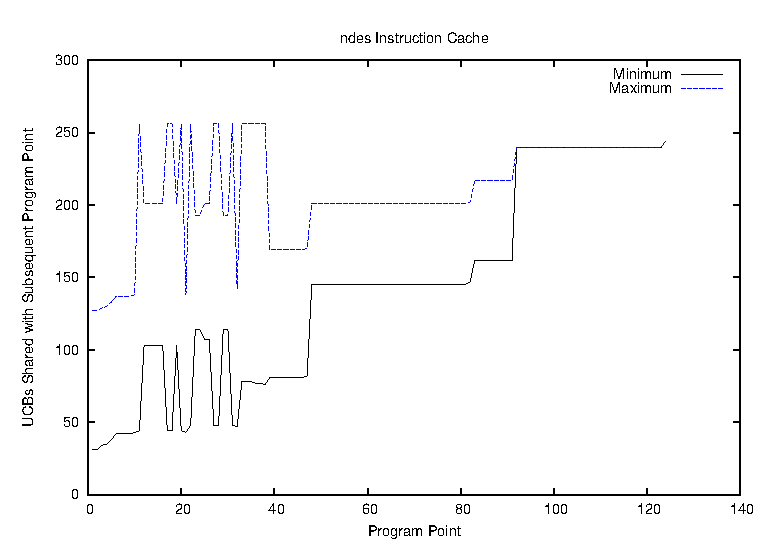
\includegraphics[width=\linewidth]{eps/ndes-icache.eps}
\caption{NDES Instruction Cache.}
\label{fig:ndes_instruction_cache}
\end{center}
\end{figure}
% 